\documentclass[l4proj.tex]{subfiles}
\begin{document}    

This chapter will look into the agile project management concepts that RViT is built upon and then examine the positive and negative aspects of three market-leading agile project management tools.

\section{Agile project management}
Agile methodology support is at the core of any project management tool designed for agile teams.

\subsection{Requirement Identification}
The agile manifesto outlines that continuous delivery of software is the highest priority and that any changes in requirements should be welcomed (\cite{Kent2001(manifesto)}). This has led to agile methodologies adopting a lightweight requirements gathering approach, where requirement identification is carried out throughout the life-cycle of a project as opposed to the traditional waterfall method where requirements are identified up front. Detailed up-front requirements analysis can lead to time being wasted as requirements may be defined and scoped that are never actually used in the project. Therefore just-in-time requirements analysis (JITRA) is often used in agile teams, to convey identified requirements into epics and user stories (\cite{Schon2017}). These epics and user stories give a user-focused view of which features are needed, while still aligning with the JITRA principle of only providing the level of detail an epic or user story requires (\cite{BHOWMIK2019}).

Good user story practises are essential to effective software development. User story templates can be used to aid teams in writing good user stories, while a definition of done can help developers understand what is required for a user story to be completed (\cite{Silva2017}).

Epic and user story mapping allows for developers to understand which story belongs to each epic. By being able to reorder these elements, developers can visually prioritise epics and user stories without having to use extremely fine-grained priority choices.

User stories can also contain a wealth of other information to help developers better understand their purpose. Category tagging can allow teams to identify which types of development a story might require, allowing for streamlined user assignment. Story points can allow teams to estimate how long user stories will take to complete, helping them to prioritise work effectively (\cite{Coelho2012}). 

From Gregory et al's research into stakeholder perceptions of business value, it was identified that project stakeholders will often have different perceptions of the business value of epics and user stories from one another (\cite{Gregory2020}). While user stories typically highlight the value of completing the relevant piece of work, this is from a user's perspective not the business's. By including a mapping from an epic or user story to the relevant business value, this will consolidate the business value of the item, leading to a clearer picture of business value for the stakeholder.

\subsection{Visualising Progress with the Kanban Framework}
%There's definitely more you could say about Kanban here. Introduce the idea of flow. The idea of WIP is to encourage a continuous flow of jobs through the board. 
Originally based on the lean manufacturing process used by Toyota, the applications of the kanban framework are far reaching (\cite{Ahmad2018}). In a software development context, the kanban framework is frequently used in both agile and DevOps environments to visualise team workflow. 

The use of kanban boards are key to this framework. This is a visualisation method that uses a set of columns to define a workflow. These workflows may change from team to team, but common column names are 'To Do', 'In Progress' and 'Done' (\cite{RadiganKanban}). Work cards, or user stories, are moved through the columns to reflect their progress, allowing for the visualisation of a team's workflow. By enabling teams to see the flow of development, kanban boards can help teams identify blockers or development bottlenecks. Teams can also use kanban boards to improve their development efficiency by identifying areas of weakness or by trying out different workflows to see what best suits their team. 

Another key aspect of the kanban framework is the idea of WIP limits. These are numerical limits that can be set on any column to limit the number of cards or user stories that can be present. These limits promote a steady flow of work by not overloading any one column. WIP limits are also good for limiting developer workflow, reducing their scope of attention to one or two user stories and preventing managers from overloading their workers with unrealistic workloads, avoiding developer burnout. There may, however, be cases when a column's WIP limit must be over-ruled, so to allow for consistent WIP limits to be maintained throughout the development of a project, developers should be able to move user stories into a column, even if this breaches the WIP limit, and appropriate visual feedback should occur to let the team know that the WIP limit has been breached.

Traditionally, in a kanban environment, as soon as a team finish one piece of work they will start work on another, leading to a continuous flow of work. However, this workflow can be adapted to work with sprints, or other project management strategies, meaning the kanban framework can be applied in many different software development environments. While the kanban framework has its roots in lean project management it is also popular with agile teams. According to the 16th State of Agile report, 56$\%$ of agile teams use kanban methodologies (\cite{StateOfAgile16}). The workflow visibility of the kanban framework also makes it suited to DevOps development, where multiple teams work on one project, meaning communication is key.


\subsection{Visible Business Values}

Epics and user stories typically have business value associated with them. However, the perceived value of an epic or user story tends to differ between stakeholders and developers (\cite{Gregory2020}). While user stories should aim to convey the value of a story using the INVEST criteria (\cite{Buglione2013}), these are often ambiguous. By defining a subset of business values, custom to a particular agile team, these can be used in epics and user stories to allow for a quick, streamlined value identification process for both stakeholders and developers. By making it easy for developers to identify business values, these should be taken into consideration during the prioritisation process and become a more integral part of an agile team's workflow. 

Highlighting the business value of an epic will also help developers understand the underlying business goal. This may affect many aspects of how the team will tackle the development of the epic. For example, if a business wants to introduce a new feature set with the goal of attracting new customers, the development team being aware that on-boarding users is the business value of the epic, this may affect how they design and/or test this new set of features. Increasing a developers understanding of the business value behind an epic or user story, can improve their perceived utility value of a task and increase their motivation to complete it (\cite{Wigfield2000}). 


\section{Existing Products}
There are many pre-existing agile project management tools on the market with considerable funding and industry backing. This selection provides a review of three industry leading tools, identifying the strengths and weaknesses of each, and explains where RViT finds its niche among these competitors.


\subsection{Jira}
Jira is a state-of-the-art project management tool, servicing over 65,000 companies across the globe (\cite{JiraUsers}). The tool offers extensive customisation options and supports a variety of agile methodologies including scrum and kanban, as seen in \textbf{Fig. \ref{fig:Jira kanban}}.
Jira also provides out-of-the-box metric reporting, which includes burndown and velocity charts, as well as cumulative flow diagrams (\cite{JiraReports}). Atlassian Open DevOps also automatically connects Jira with any of Atlassian's partner tools such as GitHub and BitBucket without the traditional overhead (\cite{JiraDevOps}). As an established tool, Jira also provides extensive documentation, not just on the application itself, but also on the agile methodologies used.

\begin{figure}[h!]
\begin{center}
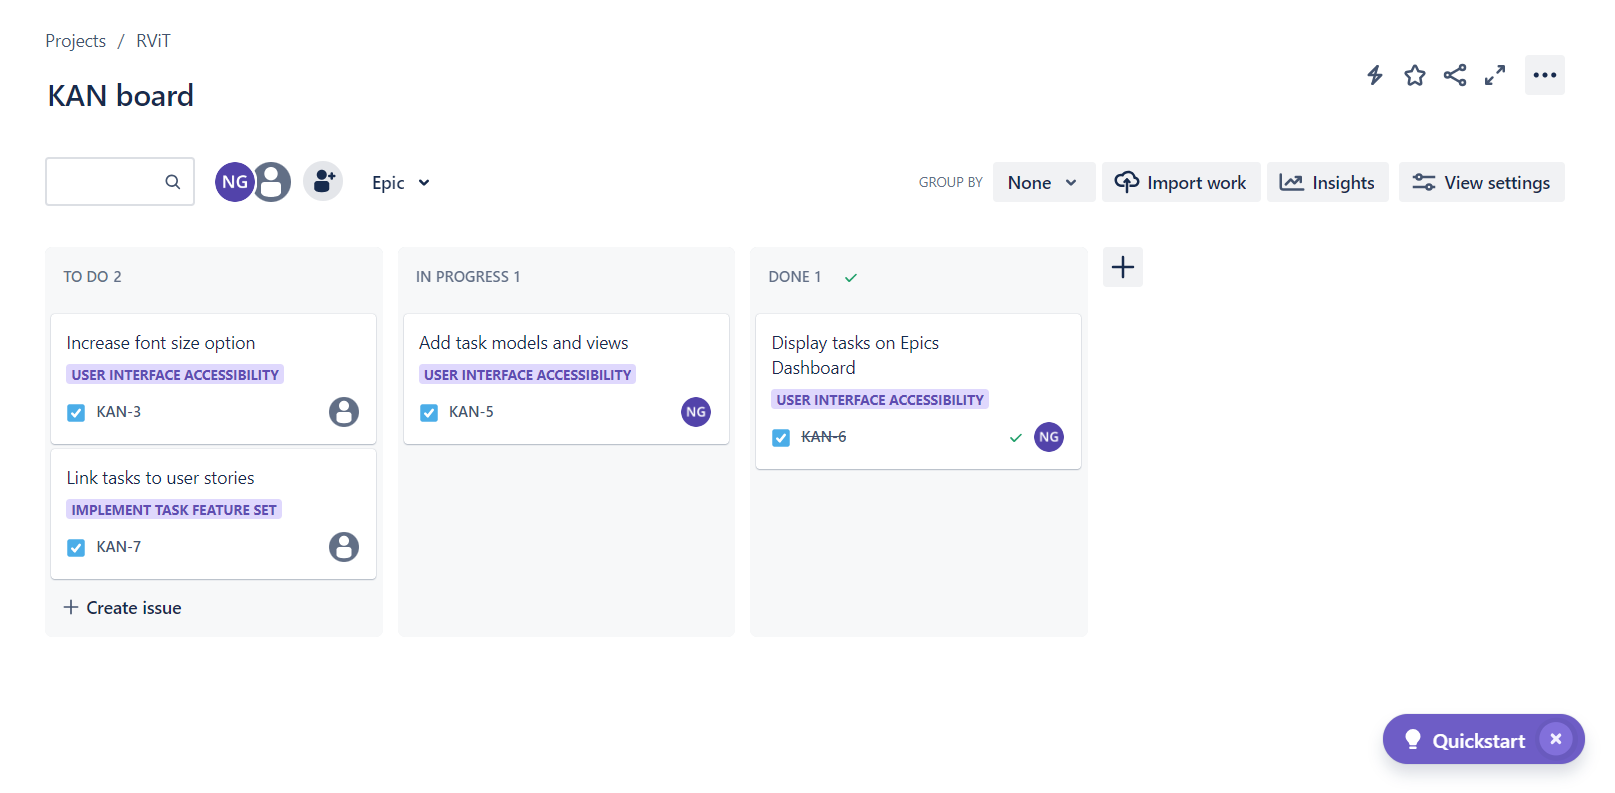
\includegraphics[scale=0.32]{dissertation/images/JiraKanbanBoard.png}
\caption{Example Jira kanban board}
\label{fig:Jira kanban} 
\end{center}
\end{figure}

As Jira is part of the Atlassian software set, the Atlassian Market place provides additional third-party Jira plug-ins and integrations to allow agile teams to further personalise their experience.  

One of the common criticisms of Jira is that the number of features it supports can be overwhelming for unfamiliar users, and leads to a steep learning curve (\cite{JiraProblemsFeatures}). The amount of customisability can also be a problem with teams sometimes creating unintuitive dashboards with no real attention paid to the developer experience (\cite{JiraProblemsFlexible}). Jira is also only free to use for teams of up to 10 developers, albeit with a slightly limited feature set. RViT aims to combat these issues by providing a free-to-use streamlined approach to kanban development that cuts out unnecessary administrative and feature overhead.


\subsection{Trello}
Trello is another Atlassian project management tool, though unlike Jira it has a significantly reduced feature set. This focuses on kanban methodology support as seen in \textbf{Fig. \ref{fig:Trello kanban}}. Another difference to Jira, is that Trello is pitched as a general project management tool as opposed to one designed for agile project management. This means typical agile methodology support such as Epic creation is not present in Trello.

Similarly to Jira, Trello also has its own marketplace where you can add third-party extensions called 'power-ups'. Power-ups can be anything from adding a priority component to a story to adding GitHub integration.

Trello is user friendly and intuitive to use with many example templates to quick start a board. However, the free version only supports the kanban board itself and not any of the other views such as the dashboard or calendar view (\cite{TrelloPricing}). RViT plans to create a similarly intuitive interface but with more out-of-the-box agile methodology support such as allowing users to create epics, define definitions of done, and add clear tags, values and priorities.


\begin{figure}[h!]
\begin{center}
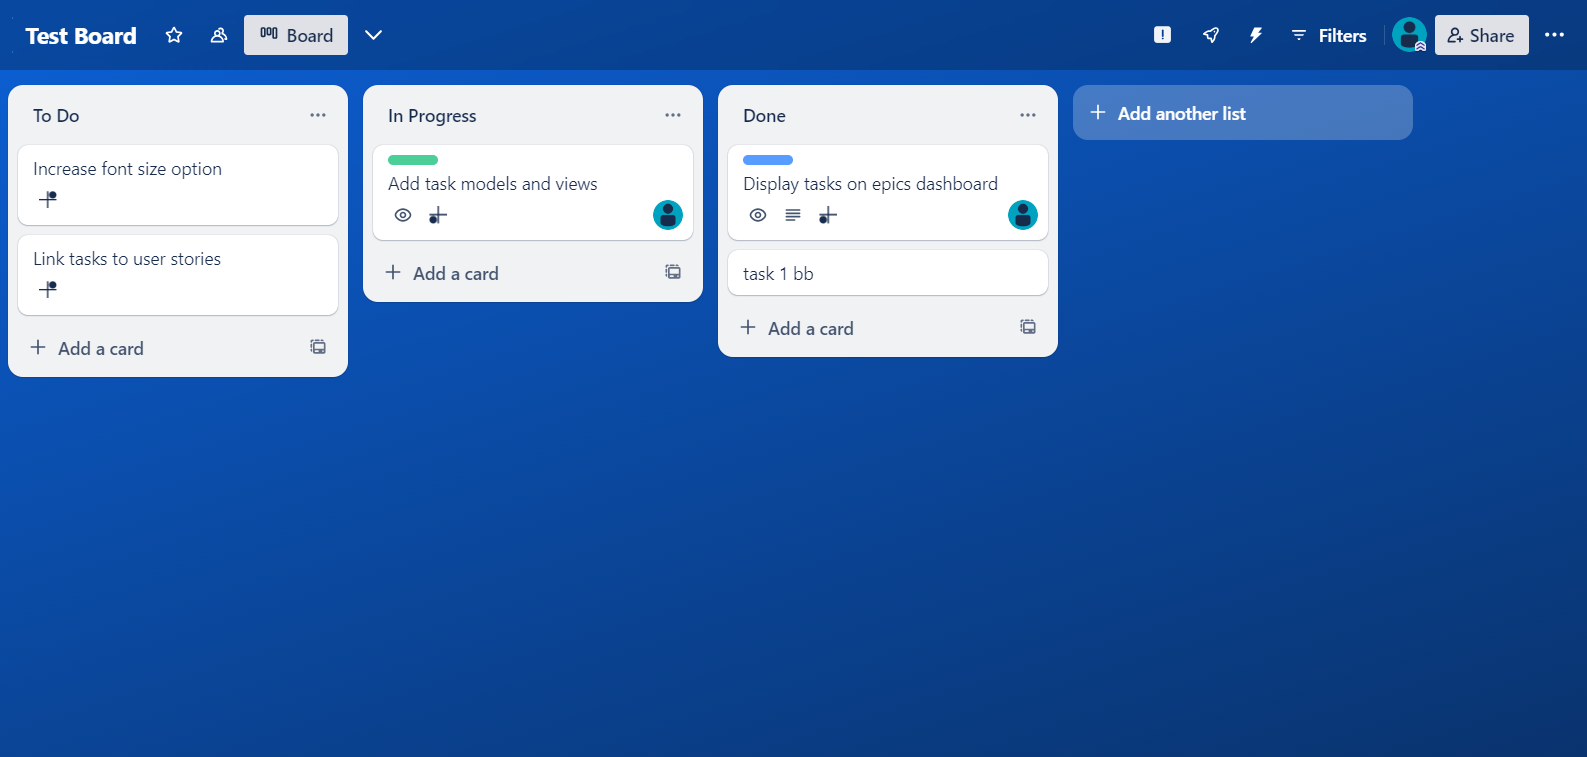
\includegraphics[scale=0.32]{dissertation/images/TrelloKanbanBoard.png}
\caption{Example Trello kanban board}
\label{fig:Trello kanban} 
\end{center}
\end{figure}

\subsection{GitHub Issues and Projects}
GitHub comes with built-in issue tracking support. Users can define issues and create custom issue templates to simplify the issue adding process. GitHub also allows developers to add customisable labels to a project and define milestones to add support for scrum-based teams. GitHub issues and projects are also accessible from the GitHub repository itself, meaning a secondary application does not have to be used. These tools are also completely free to use unlike Jira and Trello.


GitHub projects support three different views of a repository's issues, kanban board-based, table-based and roadmap-based. These views are intuitive to use but are not very visually appealing due to the lack of colour as seen in \textbf{Fig. \ref{fig:GitHub kanban}}. As well as this, the information that a developer can gain without clicking into an issue is limited, in addition to there being no support for setting issue priorities. Any labels an issue has are also not visible until the issue is clicked into.


\begin{figure}[h!]
\begin{center}
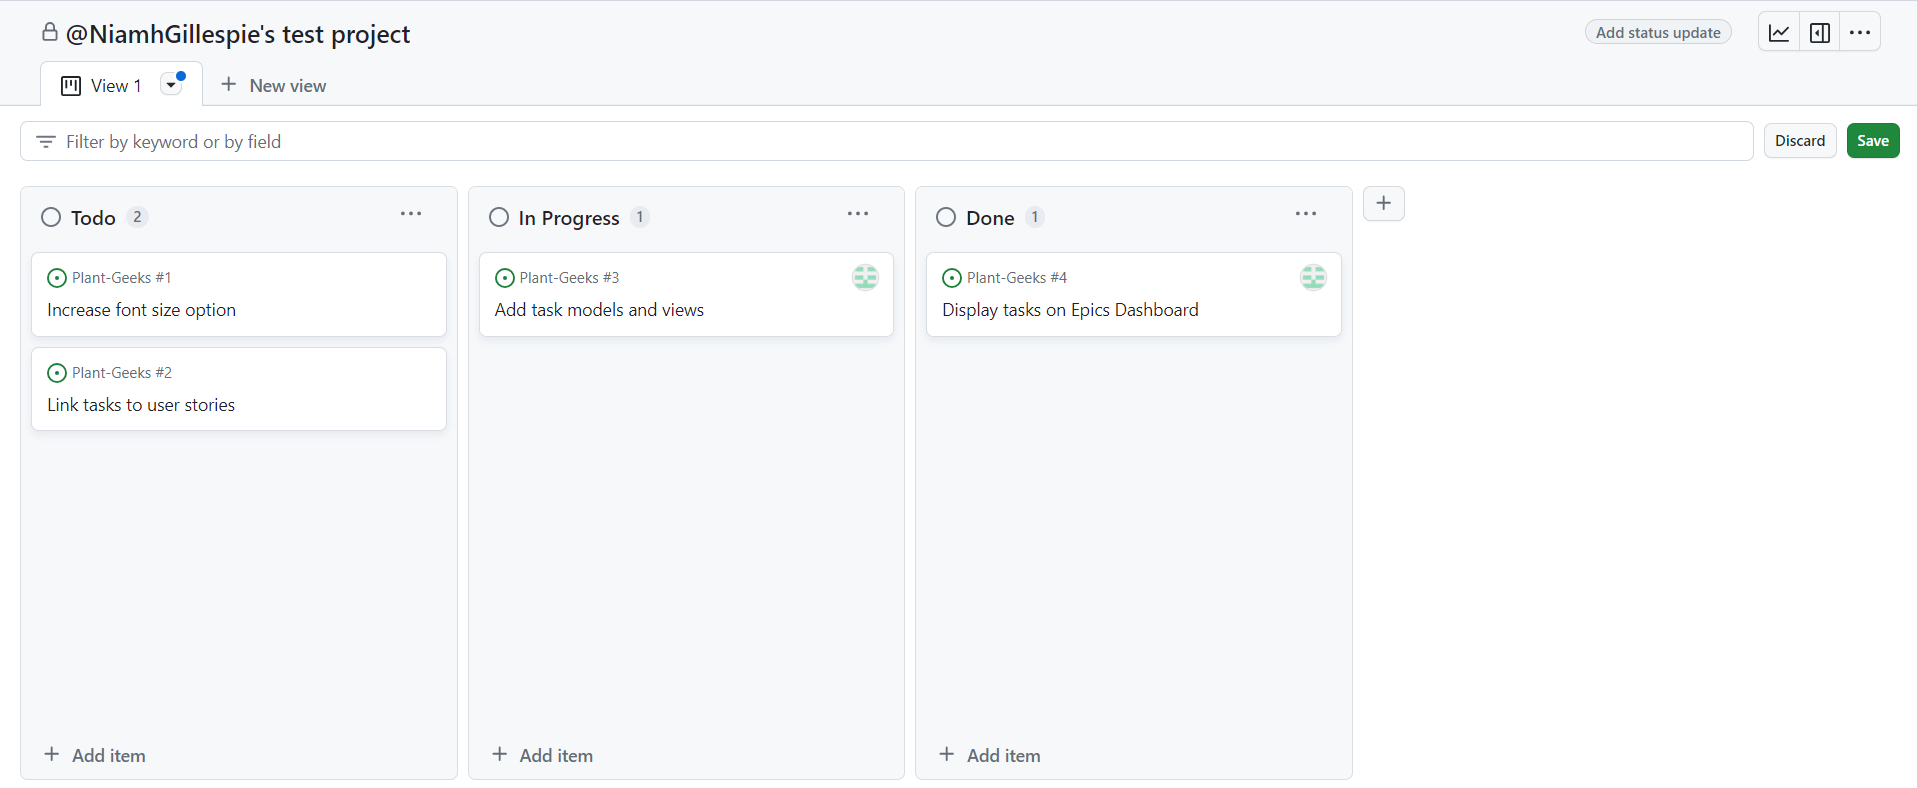
\includegraphics[scale=0.32]{dissertation/images/GitHubKanbanBoard.png}
\caption{Example GitHub kanban board}
\label{fig:GitHub kanban} 
\end{center}
\end{figure}


Like Trello, GitHub also lacks support for agile concepts like epics. RViT aims to support these concepts while also providing a more aesthetically pleasing user interface. 

\end{document}